\chapter{Experiment Implementation}
\centerline{\rule{149mm}{.02in}}
\vspace{2cm}

This chapter will cover the implementation details of the experiments, discussing the tools used, the deployment environment and other considerations made when running the data processing tasks.

\section{Choice of Data}
An important factor in big data problems is the nature of the data which is being processed. As discussed in previous chapters, data is usually large scale. It may also be unpredictable, changing in both size and quality. It is important to choose a dataset representative of what data processing tools are usually used for, as using completely synthetic data without appropriate properties will not provide an accurate portrayal of how the tools perform in the real world.

\subsection{Desirable Properties}
There are several desirable properties which will make a dataset appropriate for use in the experiments.

\subsubsection{Connectivity}
Both the Reverse Link Graph and PageRank problems treat the input data as graphs, and perform operations on them accordingly. An important property that the data must have is that the graph must have a high degree of connectivity (i.e. lots of connections between nodes in the graph). 

A Reverse Link Graph relies on a node being linked to by other nodes in the graph. In the case where there are no links between nodes, the algorithm will not generate any link pairs, and will therefore have no work to perform in the Reduce stage. The more links pairs are generated, the greater the amount of work required in the Reduce step.

In the case of PageRank, the algorithm uses values of adjacent nodes to determine a nodes value. A node which is connected to many high valued nodes will have a high value itself. This requires high degree of connectivity to provide a meaningful PageRank. It also requires that all nodes be in the graph. The subset of a graph cannot be used as it will have `dangling references' - connections where one of the nodes is outside of the graph (and therefore has no PageRank). 

\subsubsection{Size}
Size is an important property of the data as it should be reflective of real-world data sizes. In particular, the size of the data is constrained by 2 major factors.

\begin{enumerate}
	\item The size of the data cannot be too \textit{small} as it will limit the tools capacity to run the problem in parallel. Amdahl's law \cite{amdahl1967validity} states that there is a theoretical maximum speedup which can be achieved by adding additional parallel processing capacity. Past this point, adding extra resources (nodes or processors) will not result in improved runtime performance, and may detract from performance (due to additional communications overhead, or other serial factors).
	\item The size of the data cannot be too \textit{large} as there will be issues with storing, transferring, and processing the data on the resource constrained deployment environment.
\end{enumerate}

\subsubsection{Ease of Processing}
There are various different areas where Reverse Link Graph and PageRank can be used. Examples include analysing the importance of academic papers, or determining which sections of code in a program are dependant on one another. One of the major factors in choosing which type of data is used is how well suited it is to be processed by the data processing tools. 

Specifically, whilst it is possible to process other types of data, it is much simpler to process plain-text data, as there are a wide array of available input mechanisms. Both the Hadoop and Stratosphere APIs have methods of reading in a text file, processing CSVs and handling plain text in other ways. 

Many academic papers are made available in PDF format. This makes it difficult to process as custom input adaptors would have to be created to parse the data and pass it to the data processing steps. This would have limited impact on the performance of the tools, and is therefore not important within the scope of the project. 

An ideal candidate for a naturally occurring, plain text representation of a graph would be the World Wide Web. The web consists of a set of pages (nodes) with links (edges) between them. Treating the web as a graph is a common feature of other research works, including the original PageRank implementation \cite{page1999pagerank}.

\subsection{Wikipedia Datasets}
Wikipedia is an online encyclopaedia which is available in multiple languages. It exhibits all of the properties which are desirable for the data processing problems. Wikipedia represents a graph with high connectivity, as articles within the encyclopaedia often link to other articles. The Wikimedia foundation make a set of full HTML dumps available for the various language editions of Wikipedia dating up to 2008. As a plain text representation of the Wikipedia dataset, this is easier to process than alternative formats (such as PDFs). 

The various language versions of Wikipedia are different sizes. This is allows prototyping to be carried out with different data sizes, in order to find the appropriate size for the experiments.

\begin{itemize}
	\item Wiki for Schools is a charitable project aimed at providing a self-contained subset of Wikipedia for use in schools. Pages are chosen for the subset of the encyclopaedia based on whether they are part of the English school curriculum. The Wiki for Schools dataset was evaluated, but was deemed too small to provide a true test of the capabilities of the data processing tools.
	\item The Spanish language version of Wikipedia was also evaluated, but was too large to be used for data processing, as the resource constraints prevented experiments from being run on a low number of nodes.
	\item The Simple English Wikipedia is an encyclopaedia for explaining complex subjects in layman's terms, without using jargon or assuming any prior knowledge of a subject. The simple English Wikipedia provided a good compromise in data size, and was therefore chosen as the dataset for running the experiments.
\end{itemize}

\section{Data Format}
In addition to the representation of the data (a plain text representation) the underlying format used to store this data is also important. The Hadoop File System is known to suffer from the ``Small File Problem'' \cite{hdfsSmallFiles}. The file system is designed and optimised to store large files, rather than accessing lots of smaller files. In addition to this, HDFS has a large block size. Each file takes up at least one block which is by default 1MB. This will cause a significant amount of space to be wasted if each file is stored independently (as individual web pages are rarely as large as 1MB in size).

The choice was taken to pre-process the data used in the experiments in order to overcome the small file problem. Whilst this represents an inherent limitation of the technology used, it affects both Stratosphere and Hadoop equally (as both use HDFS) and therefore will not have a dramatic effect on the conclusions drawn from the experiments. It will also allow both data processing technologies a chance to perform in ideal circumstances, rather than limiting them by the choice of data. This may not reflect a real-world implementation of the processing tasks, as this pre-processing step may be prohibitively expensive in larger datasets (for example, if the whole World Wide Web was being considered).

The pre-processing step combines the small files together into a larger file, which can then be processed accordingly.

\subsection{SequenceFile}
A SequenceFile is a Hadoop-specific binary file format which stores Key/Value pairs. It is optimised for use in HDFS. A tool was created which converted an arbitrary set of web pages into a SequenceFile, by setting the key as the filename of the web page, and the value to the contents of the file. This dramatically reduced the size of the data, as it discarded irrelevant parts of the data (such as image files) and provided a more compressed representation of the text data. 

Unfortunately, the Stratosphere implementation of the SequenceFile input format was felt to be too immature for use in the experiments, and therefore the use of a SequenceFile to represent data was deemed unsuitable.

\subsection{CSV}
CSV (Comma-separated values) is a well established plain-text method of representing tabular data. While it lacks an official standard, tools which process CSV data typically follow RFC 4180 \cite{rfc4180}. As an open and accepted data format, CSV is well supported by both Hadoop and Stratosphere. The relative simplicity of the format also makes it feasible to implement a basic parser where necessary. 

Data was stored in CSV format as Key/Value pairs, with the key being the page filename, and the value being the contents of the file. This mirrors the way the data was stored in a SequenceFile, but in a more widely accepted file format. 

\section{Deployment Environment}
All experiments were run using the Leeds University School of Computing Cloud Testbed. The Cloud Testbed is a private cloud consisting of 6 machines, controlled using the OpenNebula toolkit. Virtual machines can be created as required, and this capability was used to add resources to the data processing tools. 

\begin{figure}[H]
\centering
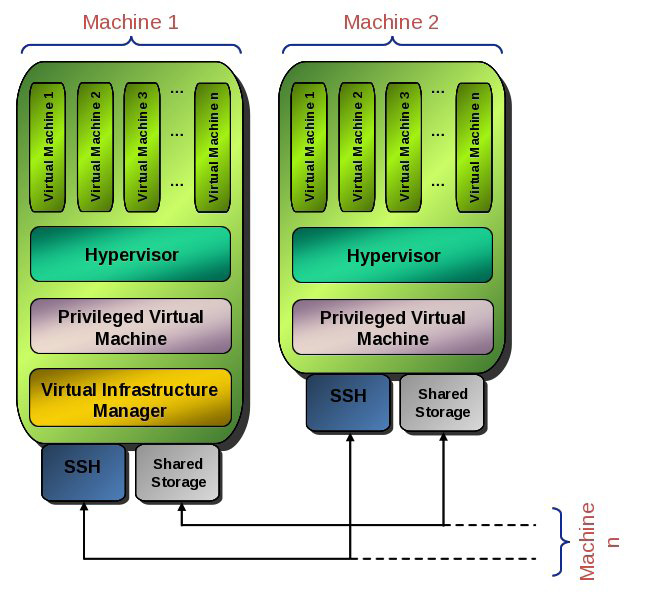
\includegraphics[scale=0.3]{resources/CloudTestBed.png}
\caption{School of Computing Cloud Testbed Architecture}
\end{figure}

\subsection{Node Specifications}
The Cloud Testbed allows the creation of Virtual Machines with fixed resources. The virtual machines are each permitted 1 virtual processor core and 1GB of memory. This allows the virtual machines to have a consistent level of performance, limiting the effect of load on the underlying hardware. The physical hardware the virtual machines execute on have Intel Xeon Quad Core processors (X3360) and 4GB of memory.

The Cloud Testbed allows for up to 10 virtual machines to be created per user. Whilst data processing software such as Hadoop has been designed to use large numbers of nodes and this cluster size may be smaller than in some real-world applications of Hadoop, significantly smaller cluster sizes are used in practice. For example, Amazon limit users of their MapReduce service to 20 nodes, and require anybody exceeding that usage to request a higher quota \cite{emrlimits}. This cluster size is consistent with previous research in the field \cite{warneke2011exploiting}.

The resources provided by the Cloud Testbed are not ideal hardware for running large scale data processing problems, which typically require large amounts of memory. Whilst this will undoubtedly impact the performance of the experiments, the environment is consistent for both Hadoop and Stratosphere, and should not affect the comparison of the tools.

\subsection{Software}
Hadoop version 2.3.0 and Stratosphere version 0.5 were installed on the cluster. At present these are the latest versions of both software packages. Stratosphere was configured to use HDFS in order to limit the effect that the file system had on the experiments. The version of Stratosphere installed was not dependent on YARN, as it was felt this would limit the effectiveness of testing scalability.

The data was loaded into HDFS before the experiments, and this was not included in runtime calculation. This limits the cost of communication overhead, as the data is already distributed across nodes appropriately, rather than data having to be transferred at the start of experiments. 

\section{Programming Language \& Frameworks}
Experiments were initially implemented in the Scala programming language \cite{scalalang}. Scala is a functional programming language with Object-Orientated support, which uses the Java Virtual Machine as a runtime environment. This allows seamless integration with existing Java libraries, such as those exposed by Stratosphere and Hadoop. As a functional language, Scala has native support for higher order functions such as map - indeed, MapReduce was originally inspired by some of the fundamental operations present in functional languages \cite{dean2008mapreduce}. This allows PACT and MapReduce jobs to be represented in a very succinct and readable manner. 

In addition to being able to call existing Java libraries, there are several `wrapper' libraries which have been developed to allow for Hadoop jobs to be written in idiomatic Scala, taking full advantage of functional features such as higher order functions. Prototypes were creating using Scalding \cite{scalding}, a library developed by Twitter, but use of this framework was later discontinued as it lacked support for later versions of Hadoop. It was replaced by Scoobi \cite{scoobi}, an open source project by NICTA.

The standard distribution of Stratosphere features a Scala API, but it was found to be too unstable for experiment development, with significant changes to the interface between different software versions. For this reason, Stratosphere experiments were reimplemented in Java, whilst reusing the core, technology agnostic processing logic which was created in Scala. 

The difference between Java and Scala is not significant in regards to processing performance. Both languages compile to Java Virtual Machine bytecode, and are therefore largely interchangeable. 
\section{Reverse Link Graph}
The Reverse Link Graph can be computed using a single Map and Reduce operation. The implementation is therefore very similar across Hadoop and Stratosphere, as it does not use any of the additional functionality present in PACT.

The Reverse Link Graph experiment was run a number of times to give an average runtime performance, as runtime can be affected by a number of external elements. 

The first step of computing the Reverse Link Graph is the Map operation. The Map stage operates on each of the documents (or articles) in the Wikipedia dataset. It extracts any HTML anchor tags from the source code of the document, and returns a list of link pairs, with the first item being the destination of the link, and the second item being the source (the current document) that the link is from.

The reduce step relies on the runtime (either Hadoop or Stratosphere) to group the items by key, so the links are grouped by the destination. The reduce step can then combine the sources into a string, giving a list of the pages which link to that destination. 

\begin{figure}[H]
\begin{tikzpicture}

% No indentation, or it'd be included on the diagram! D:

\node[doc,scale=0.5] (input) {
\begin{lstlisting}[language=html]
<html>
  <body>
    <a href="page1.htm">
      Example Article
    </a>
  </body>
</html>
\end{lstlisting}
};

\node[draw, circle, minimum size=1.5cm, right=of input] (Map) { Map };

\node[doc,scale=0.5, right=of Map] (linkpairs) {
\begin{lstlisting}
(dest1, src2)
(dest1, src3)
(dest2, src1)
(dest3, src4)
(dest3, src6)
(dest3, src7)
\end{lstlisting}
};

\node[draw, circle, minimum size=1.5cm, right=of linkpairs] (Reduce) { Reduce };

\node[doc,scale=0.5, right=of Reduce] (output) {
\begin{lstlisting}
(dest1, "src2, src3")
(dest2, "src1")
(dest3, "src4, src6, src7")
\end{lstlisting}
};

\path[->] (input) edge (Map);
\path[->] (Map) edge (linkpairs);
\path[->] (linkpairs) edge (Reduce);
\path[->] (Reduce) edge (output);

\end{tikzpicture}

\caption{A graphical representation of the Reverse Link Graph workflow}
\end{figure}

\section{PageRank}
PageRank is a more complex algorithm than the Reverse Link Graph computation, and benefits from the more advanced features of PACT. In particular as an iterative algorithm, the PageRank algorithm benefits from having iteration functionality built-in to Stratosphere. 

As Hadoop lacks some of the necessary operations to implement PageRank in an ideal way, the algorithm was implemented in twice, with the different technologies having different implementation styles. For Stratosphere, all of the features available to PACT were used, whereas with Hadoop the implementation is limited to being expressed in a MapReduce fashion.

The PageRank experiment was run a number of times to give an average runtime performance, as runtime can be affected by a number of external elements. 

For both implementations the PageRank algorithm ran for 3 iterations. This was in order to provide a fair illustration of how well iterative algorithms perform in both technologies, whilst not being prohibitively time consuming (especially on smaller cluster sizes).

\subsection{Stratosphere Implementation}
The stratosphere implementation of PageRank was the `ideal' implementation, as it has native support for a number of operations required by the PageRank algorithm. 

The first step in the process was to take the input data from the data source, and build the Reverse Link Graph. The PageRank algorithm determines the rank of a page by considering other pages which link to it, which requires the Reverse Link Graph to be computed. 

Once the Reverse Link Graph had been found, the iterative process could begin.

Each node received the PageRank of its neighbours using a Join operation, finding the scores of other nodes by their unique identifiers (the page name). The resulting data was then sent to a Reduce operation, which computed the new rank of the node by summing the rank of its neighbours, and multiplying the resulting value by a `dampening value'. 

After the first map operation, this process was applied iteratively 3 times. 

\begin{figure}[H]
\centering
\begin{tikzpicture}

% No indentation, or it'd be included on the diagram! D:
\node[circle] (dummy1) {};

\node[doc,scale=0.5, above=of dummy1] (input1) {
\begin{lstlisting}
(page1, 0.5)
\end{lstlisting}
};

\node[doc,scale=0.5, below=of dummy1] (input2) {
\begin{lstlisting}
(src1, 0.3)
(src2, 0.7)
\end{lstlisting}
};

\node[draw, circle, minimum size=1.5cm, right=of dummy1] (Join) { Join };

\node[draw, circle, minimum size=1.5cm, right=of Join] (Reduce) { Reduce };

\node[draw, right=of Reduce] (container) {

\begin{tikzpicture}
\node[rotate=90] (dots) {...};

\node (dummy2) {};

\node[doc,scale=0.5, above=of dummy2] (output1) {
\begin{lstlisting}
(page1, 0.8)
\end{lstlisting}
};

\node[doc,scale=0.5, below=of dummy2] (output2) {
\begin{lstlisting}
(src1, 0.5)
\end{lstlisting}
};

\end{tikzpicture}
};

\path[->] (input1) edge (Join);
\path[->] (input2) edge (Join);
\path[->] (Join) edge (Reduce);
\path[->] (Reduce) edge (container);
\path[arrow, dashed] (container) |- (3, 3) -| (Join);

\end{tikzpicture}

\caption{A graphical representation of the iterative part of PageRank}
\end{figure}

\subsection{Hadoop Implementation}
As Hadoop lacks the necessary operations to perform the PageRank algorithm, it must be implemented using a series of Map and Reduce operations. 

The initial process of converting the input data to the necessary format by performing the Reverse Link Graph calculation took a single Map and a Reduce operation. 

For each iteration of the algorithm, a Map and Reduce operation was required to join the node with its edges. A further MapReduce step was required to compute the updated rank for the page (as with Stratosphere). A final MapReduce step was taken to format the data in an appropriate format for the next iteration, a step taken automatically by Stratosphere.

It took a total of 10 MapReduce passes to compute the PageRank over 3 iterations.

\section{Conclusion}
This chapter has detailed the implementation concerns of the experiments. We have determined the data to be used, the runtime environment of the experiments, and the relevant data processing tool configurations. A description of the Reverse Link Graph and PageRank implementations has been given, and implementation concerns such as data format, node counts, and programming languages and frameworks used have been discussed.